In this section we will deal with the problem of positioning protein
side-chains and selecting side-chain conformations such that
the number of collisions is minimized.

As we mentioned in Section \ref{chap:protein_geometry}, statistical
analysis has shown that each type of amino acid side-chain has a small
set of common conformations \cite{dunbrack2002rotamer}. A \textit{likely} side-chain
conformation is a configuration of its $\chi$ angles and is called a
\textit{rotamer}.

There has been developed several \textit{rotamer libraries}
\cite{dunbrack1997bayesian, lovell2000penultimate}, containing lists
of the common rotamers for each side-chain together with a probability
of each of those rotamer occuring in any protein. A comparison of some,
but not the most recent, rotamer libraries can be found in
\cite{dunbrack2002rotamer}. We have selected to use the rotamer
library made by Dunbrack et al. for the SCWRL side-chain
predictor\footnote{We use the latest release from 15th May 2002. The
  library can be downloaded as \textit{bbind02.May.lib} from
  \url{http://dunbrack.fccc.edu/bbdep/bbdepdownload.php}}.

\section{Our approach}
\begin{figure}
    \centering
    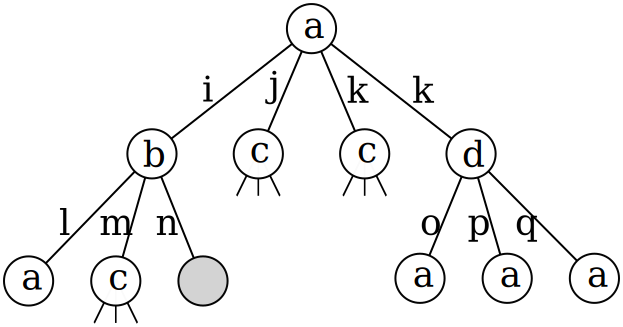
\includegraphics[width=.9\columnwidth]{figures/rotamersearch}
    \caption{The structure of our rotamer search space when
      eliminating collisions with the amino acid \textit{a}. Edges
      represents collisions and they are labelled with the rotamer
      that performed the collision. Following the path from \texit{a}
      to the grey node and applying the rotamers represented by edges
      will resolve the collision.
    \label{fig:rotamer-search-tree}
\end{figure}
We have devised a simple algorithm for the rotamer selection problem.
The first step of our algorithm is to decide on an initial state with
as few collisions to handle as possible. We obtain this by
initializing the amino acids with their most propable rotamer from the
rotamer library. The algorithm then iterates through the amino acids
and solves \textit{local} collision problems. That is, we search for a
rotamer configuration that can eliminate collisions involving the
current amino acid or at least reduce the number of collidees. We can
illustrate this search for collisionless rotamers by a tree that
represents the eventual collisions occuring for each choice of rotamer
for the current amino acid and choice of rotamers for its
collidees. In Figure
\ref{fig:rotamer-search-tree} we have shown such a tree, for the
situation where we want to remove collisions with a single amino acid,
\textit{a}. Each vertex represents an amino acid and each edge
represents a collision between the node and its child. The names on
the edges represents rotamers of the node above. For example, when the
rotamer $3$ is applied to amino acid \textit{a}, \textit{a} collides
with both \textit{c} and \textit{d} and no matter which of the three
available rotamers for \textit{d} that is used, \textit{d} will always
collide with \textit{a}. A solution is found when the application of a
rotamer to an amino acid has no collidees. For example, we can
eliminate the collision in the figure by using rotamer $1$ for amino
acid \textit{a} and rotamer $3$ for amino acid
\textit{b}. The solution is marked with grey in the figure.
We use a breadth-first search through this tree, visiting
each level down to some maximum depth. The edges are followed in order
of rotamer-probability, such that the most probable rotamer are
visited first (left-to right in the figure). We continue through the
tree until a solution is found or the maximum depth is reached.

In cases where an amino acid collides with more than one
other amino acid, we stop as soon one of the collisions is solved and
postpone the solution of the remaining collisions to we reach one of
the collidees we have not handled.

%% Hvornår kigger vi på rotameren som /a/ startede ud med at have?

\section{Related Work}
The side-chain positioning (SCP) problem has been investigated by
several research groups, what we found most notably is the work done
by Dunbrack Labs on the SCWRL project \cite{canutescu2003graph,
  krivov2009improved}. The central algorithm in SCWRLs collision
resolving uses an \textit{interaction graph}, which much like our tree
has a vertex for each amino acid, but instead of the edges
representing that there currently is a collision, the graph has edges
between two amino acids if they \textit{could} collide by applying
certain rotamers on either or both of the amino acids. This graph can
be used to find clusters of interacting residues (two residues can
interact if there is a path between them). Large clusters can not be
solved efficiently, but a cluster can be partitioned if there exists
what is called \textit{keystone vertices} or \textit{articulation
  points} which when removed breaks the graph into two separate
subgraphs. For each rotamer of the keystone residue the two
subproblems can be solved. The rotamer of the keystone residue which
results in the lowest amount of free energy for the complete cluster,
is selected for the amino acid. Remark here that they use energies to
evaluate the best rotamer whereas we have limited us from dealing
with energy functions and instead concentrate on the number of
collisions.

In addition to this central algorithm, SCWRL has further advantages
over our algorithm. They use a lot of effort to delimit their search
space e.g. by removing rotamers with high self-energy from the set of
possible rotamers, whereas we have not focused at all on performance
in our implementation. SCWRL also tries to resolve whether any
collisions can be transformed into disulfide bridges, which are bonds
between two cysteine amino acids from different places on the amino
acid sequence but spatially near each other (only pairs of cysteine
residues can form disulfide bridges). We limited ourselves from this
problem from the beginning.

C. L. Kingsford et al. \cite{kingsford2005solving} defines the problem
in a somewhat different way than the team behind SCWRL. Their graph
representation contains vertices for each rotamer of each residue and
they introduce weights on the graph that represents the energies it
would incur to select the rotamer configuration represented by an
edge. A solution to the problem is a selection of rotamers, such that
all amino acids has exactly one rotamer. They state this problem as a minimization
problem that can be solved by linear programming. Their first attempt
at solving the problem relaxes the integrality constraint on the
rotamer selection, which can be solved by linear programming. If this
does not return a solution where all values are integral they have to
solve the harder, unrelaxed definition of the problem using integer
programming.

%%% Local Variables: 
%%% mode: latex
%%% TeX-master: "rapport"
%%% End: 
